\section{Results IV: variance features from 5-minute data}\label{sec:rv}

The SMoE's variance covariates are built from the daily high--low range because the range is
available for every series and every day. For the CSI~300 we also have 5-minute bars, and realised
variance from intraday returns is the textbook measure of daily variance
\citep{andersen2003modeling}. This section asks whether the conclusions change when the range is
replaced by realised measures, and it turns the comparison into a test of a measurement-error
prediction that the white box makes possible.

\subsection{Theory: what a better variance measure should change}

Let $\ell_t=\log\sigma^2_t$ denote the latent log variance of day $t$'s trading session. Every daily
estimator we use has the multiplicative form $\hat v_t=\sigma^2_t\varepsilon_t$, so
\begin{equation}\label{eq:logmeas}
  \log\hat v_t=\ell_t+\kappa+\eta_t,\qquad \E\eta_t=0,\quad \Var\eta_t=\omega^2,
\end{equation}
with $\eta_t$ independent of $\{\ell_s\}$. Under a Brownian semimartingale with constant intraday
volatility and no microstructure noise, $\varepsilon_t$ has a known law. For the squared daily
return $\varepsilon_t\sim\chi^2_1$ and $\omega^2=\psi'(1/2)=\pi^2/2\approx4.93$, where $\psi'$ is the
trigamma function. For realised variance from $M$ intraday returns
$\varepsilon_t\sim\chi^2_M/M$, so $\kappa=\psi(M/2)-\log(M/2)$ and $\omega^2=\psi'(M/2)\approx2/M$;
with $M=48$ five-minute returns, $\omega^2=0.043$. For the Parkinson estimator $\varepsilon_t$ is the
squared range of a standard Brownian motion on $[0,1]$ divided by $4\log2$; its log-variance has no
simple closed form and we compute it by simulation (\cref{tab:rv-measure}). Microstructure noise and
the intraday volatility pattern raise the effective $\omega^2$ of both intraday estimators
\citep{hansen2006realized}, which is why we also estimate it from the data.

\paragraph{What a log-variance error costs.}
The cost of a variance error in log score has a simple exact form.

\begin{lemma}[Cost of a log-variance error]\label{lem:logvar-cost}
Let $y\sim\N(\mu,\sigma^2)$ and let the forecast be $\N(\mu,s^2)$ with $u=\log(s^2/\sigma^2)$. Then
\begin{equation}\label{eq:logvar-cost}
  \E\big[-\log\varphi(y;\mu,s^2)\big]-\E\big[-\log\varphi(y;\mu,\sigma^2)\big]=\tfrac12\big(u+e^{-u}-1\big)
  =\tfrac{u^2}{4}-\tfrac{u^3}{12}+O(u^4),
\end{equation}
which is one half of the QLIKE loss of $s^2$ evaluated at the true variance. If $u$ is random with
mean $b$ and variance $v$, independent of $y$ given $\sigma^2$, the expected excess log score is
$\tfrac14(b^2+v)$ to second order.
\end{lemma}

\noindent The lemma converts the measurement problem into a forecasting prediction: a variance
covariate that lowers the variance of the log-variance forecast error by $\Delta v$ should improve the
average log score by about $\Delta v/4$ nats per day. It also explains why log score and QLIKE rank
variance forecasts identically to second order.

\paragraph{Where the measurement error goes.}
The variance covariates enter through the log-HAR vector
$\bv_t=(\log\hat v_t,\log\bar v^{(5)}_t,\log\bar v^{(22)}_t)$. Averaging over five or twenty-two days
removes most of $\eta$, so the error sits mainly in the daily component. Let
$\bv^\ast_t=(\ell_t,L^{(5)}_t,L^{(22)}_t)$ be the latent counterparts with covariance $\Sigma^\ast$,
let $\bm b$ and $\nu_1$ be the coefficients and residual variance of the linear projection of $\ell_t$
on $(L^{(5)}_t,L^{(22)}_t)$, and let $\bm\delta=(\delta_1,\delta_5,\delta_{22})$ be the slopes of the
projection of the target log variance on $(1,\bv^\ast_t)$.

\begin{proposition}[Errors in the variance regressors]\label{prop:eiv}
If $\bv_t=\bv_t^\ast+\kappa\bm1+\bm\xi_t$ with $\bm\xi_t$ independent of $\bv^\ast$ and of the
target, $\E\bm\xi_t=\bm0$ and $\Var\bm\xi_t=\Sigma_\xi$, the slopes of the projection on the observed
covariates are $\bm\delta^{\mathrm{obs}}=(\Sigma^\ast+\Sigma_\xi)^{-1}\Sigma^\ast\bm\delta$. If the error is
confined to the daily component, $\Sigma_\xi=\omega^2\bm e_1\bm e_1^\top$, then
\begin{equation}\label{eq:eiv}
  \delta_1^{\mathrm{obs}}=\frac{\nu_1}{\nu_1+\omega^2}\,\delta_1,\qquad
  \delta_h^{\mathrm{obs}}=\delta_h+\frac{\omega^2}{\nu_1+\omega^2}\,b_h\,\delta_1\quad(h=5,22),
\end{equation}
and the sum of slopes changes by $-\frac{\omega^2}{\nu_1+\omega^2}\delta_1(1-b_5-b_{22})$.
\end{proposition}

\noindent Three predictions follow. First, the daily loading is attenuated by
$\nu_1/(\nu_1+\omega^2)$, where $\nu_1$ is not the variance of daily log variance but the much smaller
part of it that weekly and monthly averages do not explain. Even a modest $\omega^2$ can therefore
remove most of the daily loading. Second, the lost weight moves to the weekly and monthly components
in proportion to how well they predict the daily one, so a noisy daily measure makes volatility look
like a slower process than it is. Third, when $b_5+b_{22}\approx1$, as for a persistent log variance,
total persistence is almost unchanged: measurement error re-allocates weight across horizons rather
than removing it. Comparing a range-based and a realised-variance fit gives the testable ratio
\begin{equation}\label{eq:eiv-ratio}
  \frac{\delta_1^{\mathrm{PK}}}{\delta_1^{\mathrm{RV}}}=\frac{\nu_1+\omega^2_{\mathrm{RV}}}{\nu_1+\omega^2_{\mathrm{PK}}}.
\end{equation}
The SMoE's variance equation is a log-link Gamma regression rather than a linear projection, so
\eqref{eq:eiv} holds there to the order of the regression-calibration approximation
\citep{carroll2006measurement}; we check it on the $K=1$ model and on each expert.

\paragraph{Specifications.}
We estimate six SMoE variants that differ only in the variance covariates and the volatility
state of the gate. SMoE-PK is the baseline. SMoE-RV replaces the three range components by the
log-HAR of realised variance and the gate's volatility state by $\log\overline{\mathrm{RV}}^{(22)}$.
SMoE-TV adds the squared overnight return to realised variance, because the target is a
close-to-close return and the trading-session measures miss the overnight gap. SMoE-CJ splits
realised variance into a continuous part, measured by bipower variation \citep{barndorff2004power},
and a jump term $\log(1+J_t)$ with $J_t=\max(\mathrm{RV}_t-\mathrm{BV}_t,0)$, in the spirit of the
HAR-CJ model \citep{andersen2007roughing,corsi2010threshold}. SMoE-SV uses the negative and positive
realised semivariances of day $t$ in place of the daily component, following \citet{patton2015good},
who find that ``bad'' volatility predicts future volatility more strongly than ``good'' volatility.
SMoE-PKRV includes both range and realised components, so it encompasses SMoE-PK and SMoE-RV. The
benchmarks are the $K=1$ versions of SMoE-PK and SMoE-RV, GARCH-$t$, and the log-linear Realized
GARCH of \citet{hansen2012realized} with Student-$t$ errors,
\begin{equation}\label{eq:rgarch}
  r_t=\mu+\sqrt{h_t}z_t,\quad \log h_t=\omega+\beta\log h_{t-1}+\gamma\log\mathrm{RV}_{t-1},\quad
  \log\mathrm{RV}_t=\xi+\phi\log h_t+\tau_1z_t+\tau_2(z_t^2-1)+u_t,
\end{equation}
which is the standard way to bring realised measures into a return density and is estimated by
maximising the joint likelihood of $(r_t,\log\mathrm{RV}_t)$.

We use the CSI~300 and the two instruments written on it, the IF futures and the 510300 ETF; all
three use the index's realised measures. Every model is re-estimated on the same rows (days with
5-minute data) in the same quarterly walk-forward, from the first quarter with 750 training days to
the end of the development period. The 5-minute data cover only 246 lockbox days, so the lockbox is
not used here.

\subsection{The measurement-error prediction holds}

\Cref{tab:rv-measure} puts numbers on \cref{prop:eiv}. Under Brownian motion the log Parkinson
estimator has $\omega^2=0.337$; the value implied by the data, from the residual variance of the daily
range on its weekly and monthly averages, is $0.350$. The two agree closely, so the index's daily
range behaves almost exactly like the range of a Brownian path. Realised variance has
$\omega^2=0.043$. The residual variance of daily log variance given its weekly and monthly averages
is only $\nu_1=0.146$, and this small denominator is what makes the range costly: the attenuation
factor $\nu_1/(\nu_1+\omega^2)$ is $0.30$ for the range and $0.77$ for realised variance.
Equation \eqref{eq:eiv-ratio} then predicts $\delta_1^{\mathrm{PK}}/\delta_1^{\mathrm{RV}}=0.39$ (or
$0.38$ with the data-implied $\omega^2$). In the $K=1$ model the estimated daily loadings are $0.169$
(s.e.\ $0.059$) with the range and $0.424$ (s.e.\ $0.098$) with realised variance, a ratio of $0.40$
(\cref{fig:rv-har}).

The other two predictions hold in the direction stated. With the range, the weekly and monthly
loadings are larger ($0.131$ and $0.606$ against $0.066$ and $0.403$), so the noisy daily measure
makes CSI~300 volatility look slower than it is, and the sum of the three loadings is almost
unchanged ($0.906$ against $0.893$). The proposition puts the shifted weight on the weekly component
($b_5=0.96$, $b_{22}\approx0$), whereas the estimates move it mainly to the monthly one. The weekly
and monthly components are highly collinear and their loadings have standard errors of $0.08$ to
$0.11$, so this split is not well determined. Inside the three-expert SMoE the expert-specific daily
loadings are too imprecise for the ratio to be informative, and we do not interpret them.

\begin{table}[!htbp]\centering\small
\caption{Measurement error of daily variance estimators and the implied attenuation of the daily HAR loading (CSI 300, development sample)}\label{tab:rv-measure}
\begin{adjustbox}{max width=\textwidth}
\begin{tabular}{lrr}
\toprule
Daily estimator & $\omega^2=\Var\eta_t$ & $\nu_1/(\nu_1+\omega^2)$\\
\midrule
squared return & 4.935 & 0.029\\
Parkinson range (BM) & 0.337 & 0.303\\
Parkinson range (implied) & 0.350 & 0.295\\
5-min RV (M=48) & 0.043 & 0.775\\
\bottomrule
\end{tabular}
\end{adjustbox}
\par\smallskip\begin{minipage}{\textwidth}\footnotesize
$\omega^2$ for squared returns and RV from the $\chi^2$ laws in the text; Parkinson (BM) by simulation of 20,000 Brownian paths with 2,400 steps; Parkinson (implied) from the residual variance of the daily range on its weekly and monthly averages minus $\nu_1$. $\nu_1=0.146$ is the residual variance of daily log RV on its weekly and monthly averages minus $\omega^2_{\mathrm{RV}}$; projection coefficients $b_5=0.958$, $b_{22}=-0.002$. Predicted $\delta_1^{\mathrm{PK}}/\delta_1^{\mathrm{RV}}$ from \eqref{eq:eiv-ratio}: 0.39 (BM) and 0.38 (implied); estimated in the $K=1$ model: 0.40.
\end{minipage}
\end{table}

\begin{figure}[t]\centering
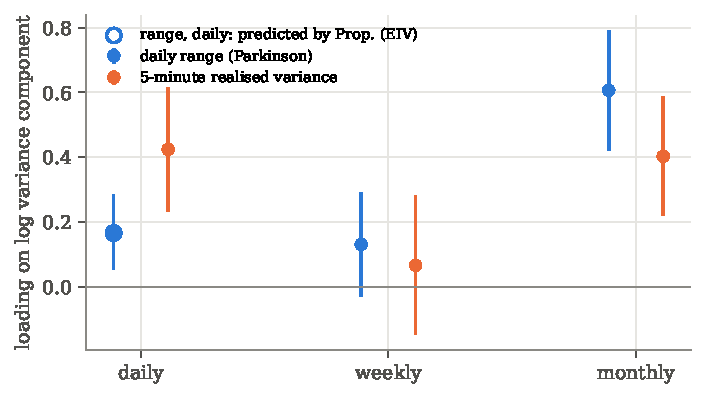
\includegraphics[width=0.78\textwidth]{../results/figures/rv_har_loadings.pdf}
\caption{Log-HAR loadings of the $K=1$ model for CSI~300 with range-based and realised daily variance
(95\% intervals from sandwich standard errors). The hollow circle is the range-based daily loading
predicted by \cref{prop:eiv} from the realised-variance estimate and the measurement-error variances of
\cref{tab:rv-measure}.}\label{fig:rv-har}
\end{figure}

\subsection{Out-of-sample results}

\Cref{tab:rv-oos} reports the walk-forward comparison. Four results stand out.

\emph{Realised measures improve the SMoE everywhere, modestly.} Each of the five realised-variance
specifications has a better log score than SMoE-PK on each of the three series (15 of 15
comparisons). The gains range from $0.14$ to $1.61$ hundredths of a nat per day and are significant
in 4 of the 15 comparisons. They are clearer for the variance forecast itself: on the CSI~300 every
realised specification has a significantly lower QLIKE than SMoE-PK, and against the 5-minute proxy
QLIKE falls from $0.331$ to $0.289$--$0.306$ and the Mincer--Zarnowitz $R^2$ rises from $0.19$ to
$0.34$--$0.36$ (except for SMoE-CJ, whose $R^2$ of $0.11$ illustrates how fragile that statistic is on
variance levels). The refinements of SMoE-RV add little: the overnight term (TV), the jump split
(CJ), the semivariances (SV) and the encompassing model (PKRV) all lie within one hundredth of a nat
of SMoE-RV on every series.

\emph{The mixture still adds to a single regime.} With realised covariates on both sides, SMoE-RV has
a significantly better log score than the single-regime Gauss-HAR-RV on all three series (one-sided
$p\approx0.02$ in each case), and the single-regime models fail the 1\% Kupiec test on more series.
The size of the mixture's advantage shrinks, however, from $0.022$ nats per day with range-based
covariates to $0.016$ with realised ones, a point we return to below.

\emph{A single-regime model with realised variance is the best density forecaster here.} The
log-linear Realized GARCH with Student-$t$ errors has the best log score on all three series. It
beats SMoE-PK significantly everywhere and SMoE-RV significantly on the CSI~300 ($p<0.001$) and the
ETF ($p=0.008$), but not on the IF futures ($p=0.17$). On QLIKE and on the FZ0 tail losses it is
statistically indistinguishable from SMoE-RV, and the 10\% model confidence set for log score keeps
every model except the range-based Gauss-HAR on all three series. We report this result plainly: once a
precise variance measure is available, a GARCH recursion that uses it with fat-tailed errors is
at least as good as three readable regimes, and on two of three series better.

\emph{\Cref{lem:logvar-cost} explains most of the single-regime gains and why the mixture gains less.}
\Cref{tab:rv-lemma} compares the log-score difference predicted from the accuracy of each model's
variance forecast, $\Delta\Var(e_t)/4$, with the difference observed. For the single-regime pair the
prediction is close: $-1.01$ against $-1.15$ hundredths of a nat when the range is replaced by
realised variance; for Realized GARCH it is $-2.43$ against $-2.08$. For the SMoE the observed gains
are roughly a third of the prediction ($-0.49$ against $-1.34$ for SMoE-RV). The lemma assumes a
Gaussian predictive; a scale mixture is less sensitive to an error in its overall variance because
its components already spread probability over several variance levels. Part of the mixture's
advantage in the main results is therefore insurance against a noisy variance covariate, and that
part shrinks when the covariate improves. This is consistent with the smaller mixture advantage
noted above.

\begin{table}[!htbp]\centering\footnotesize
\caption{Realised-variance covariates out of sample (development period)}\label{tab:rv-oos}
\begin{adjustbox}{max width=\textwidth}
\begin{tabular}{lrrrrrrrr}
\toprule
Model & CSI NLL & CSI QLIKE & CSI FZ5 & IF NLL & ETF NLL & QLIKE$_{\mathrm{RV}}$ & MZ $R^2_{\mathrm{RV}}$ & Kupiec 1\%\\
\midrule
SMoE-PK & 1.5727 & 1.5848 & 1.0246 & 1.4866 & 1.4796 & 0.331 & 0.189 & 3\\
SMoE-RV & $-0.49$ & $-2.93^{*}$ & $-1.82$ & $-1.21$ & $-0.97^{*}$ & 0.291 & 0.351 & 3\\
SMoE-TV & $-0.14$ & $-2.42^{*}$ & $-0.72$ & $-0.92$ & $-0.79$ & 0.306 & 0.358 & 3\\
SMoE-CJ & $-0.31$ & $-2.33^{*}$ & $-1.37$ & $-1.50^{*}$ & $-1.08^{*}$ & 0.300 & 0.112 & 3\\
SMoE-SV & $-0.56$ & $-2.12^{*}$ & $-1.70$ & $-1.61^{*}$ & $-0.56$ & 0.289 & 0.338 & 3\\
SMoE-PKRV & $-0.26$ & $-1.79^{*}$ & $-1.00$ & $-0.71$ & $-0.58$ & 0.304 & 0.343 & 3\\
Gauss-HAR-PK & $2.21$ & $-0.67$ & $0.19$ & $0.82$ & $2.43$ & 0.317 & 0.270 & 2\\
Gauss-HAR-RV & $1.06$ & $-3.02^{*}$ & $-1.72$ & $0.17$ & $1.38$ & 0.286 & 0.326 & 1\\
GARCH-t & $-0.51$ & $1.54$ & $1.04$ & $-0.92$ & $-1.02^{*}$ & 0.350 & 0.237 & 3\\
RealGARCH-t & $-2.08^{*}$ & $-3.32^{*}$ & $-1.98$ & $-1.95^{*}$ & $-2.24^{*}$ & 0.272 & 0.401 & 2\\
\bottomrule
\end{tabular}
\end{adjustbox}
\par\smallskip\begin{minipage}{\textwidth}\footnotesize
First row: SMoE-PK losses. Other rows in loss columns: loss of SMoE-PK minus loss of the model, $\times100$ (positive = model better); $^*$: one-sided DM-HLN $p<0.05$ in favour of the model. QLIKE$_{\mathrm{RV}}$ and MZ $R^2_{\mathrm{RV}}$: CSI 300 variance forecasts against $\mathrm{RV}_{t+1}+r^2_{\text{overnight},t+1}$. Kupiec 1\%: series (of 3) on which the 1\% VaR passes at 5\%. Common samples: CSI 300 $n=2850$, IF $n=904$, ETF $n=2062$.
\end{minipage}
\end{table}
\begin{table}[!htbp]\centering\small
\caption{Log-score gains predicted by \cref{lem:logvar-cost} from the accuracy of the variance forecast, CSI 300}\label{tab:rv-lemma}
\begin{adjustbox}{max width=\textwidth}
\begin{tabular}{lrrr}
\toprule
Model & $\Var(e_t)$ & Predicted $\Delta$NLL & Observed $\Delta$NLL\\
\midrule
SMoE-PK & 0.465 & 0.000 & 0.000\\
SMoE-RV & 0.412 & -1.336 & -0.490\\
SMoE-TV & 0.429 & -0.898 & -0.141\\
SMoE-CJ & 0.418 & -1.176 & -0.308\\
SMoE-SV & 0.419 & -1.148 & -0.560\\
SMoE-PKRV & 0.435 & -0.757 & -0.259\\
Gauss-HAR-PK & 0.441 & -0.594 & 2.206\\
Gauss-HAR-RV & 0.401 & -1.604 & 1.055\\
GARCH-t & 0.485 & 0.491 & -0.509\\
RealGARCH-t & 0.368 & -2.428 & -2.083\\
\bottomrule
\end{tabular}
\end{adjustbox}
\par\smallskip\begin{minipage}{\textwidth}\footnotesize
$e_t=\log(\mathrm{RV}_{t+1}+r^2_{\text{overnight},t+1})-\log\hat V_t$, with $\hat V_t$ the forecast variance. Predicted $\Delta$NLL $=\{\Var(e_t)-\Var(e_t^{\text{SMoE-PK}})\}/4$; observed $\Delta$NLL is the out-of-sample log-score difference from SMoE-PK. Both $\times100$, nats per day; negative = better than SMoE-PK. The error of the proxy is common to all models and cancels.
\end{minipage}
\end{table}

\subsection{In-sample white box}

\Cref{tab:rv-insample} re-estimates the CSI~300 SMoE on the days with 5-minute data (June 2009 to
June 2024). Realised covariates raise the log-likelihood by 16.6 (SMoE-RV) and 21.4 (SMoE-TV) points
at the same number of parameters, and BIC selects SMoE-TV. Two of the white-box conclusions of
\cref{sec:results-china} survive the change of variance measure and one weakens. Momentum and drawdown
remain absent from the gate under every specification ($p$ between $0.24$ and $0.45$). The
volatility effect in the gate is weaker on this shorter sample, which starts after the 2007--08
boom and bust: the Wald statistic is $6.5$ ($p=0.04$) with the range, $3.4$ ($p=0.19$) with
trading-session realised variance and $14.6$ ($p<0.001$) when overnight variance is included.
Volatility is still the only candidate regime variable, but how strongly it moves the gate depends on
whether the overnight gap is measured. Finally, the semivariance model does not support the
asymmetry that \citet{patton2015good} find for US stocks: the hypothesis that negative and positive
semivariances have equal loadings in all three experts is not rejected ($W=1.42$, $p=0.70$).

\begin{table}[!htbp]\centering\small
\caption{In-sample fits with range-based and realised variance covariates, CSI 300 (June 2009--June 2024, days with 5-minute data)}\label{tab:rv-insample}
\begin{adjustbox}{max width=\textwidth}
\begin{tabular}{lrrrrr}
\toprule
Model & Log-lik. & Params & BIC & $W$ vol. in gate & $W$ mom.+dd in gate\\
\midrule
SMoE-PK & -5857.5 & 27 & 11,937 & 6.54 (0.038) & 5.53 (0.237)\\
SMoE-RV & -5841.0 & 27 & 11,903 & 3.35 (0.187) & 5.31 (0.257)\\
SMoE-TV & -5836.1 & 27 & 11,894 & 14.56 (0.001) & 3.86 (0.425)\\
SMoE-CJ & -5845.9 & 30 & 11,938 & 1.11 (0.574) & 4.71 (0.318)\\
SMoE-SV & -5839.5 & 30 & 11,925 & 6.46 (0.040) & 3.66 (0.454)\\
SMoE-PKRV & -5829.8 & 36 & 11,955 & 1.33 (0.515) & 4.66 (0.324)\\
Gauss-HAR-PK & -5999.5 & 9 & 12,073 & -- & --\\
Gauss-HAR-RV & -5960.8 & 9 & 11,995 & -- & --\\
\bottomrule
\end{tabular}
\end{adjustbox}
\par\smallskip\begin{minipage}{\textwidth}\footnotesize
Robust Wald statistics ($p$-values) that the volatility state (2 df) and the momentum and drawdown states (4 df) are absent from the gate. Equality of the negative and positive semivariance loadings in all three experts of SMoE-SV: $W=1.42$ (3 df, $p=0.70$).
\end{minipage}
\end{table}

\paragraph{Implications.} The regime structure and the precision of the variance measure are partly
substitutes: a better measure reduces the gain from mixing without removing it. The main results,
which use the range for every series, therefore understate what any model with a precise variance
measure achieves, and they somewhat overstate the share of the SMoE's advantage that is due to its
regimes. Where intraday data exist, the natural next step is an SMoE whose
experts have Realized-GARCH-type variance recursions, which would combine the readable regimes with
the variance dynamics that won here (\cref{sec:agenda}).
